%% Standalone lecture -- build with:  pdflatex -shell-escape sgd
%% Shared preamble for standalone lecture files.
%%
%% Every lecture begins with %% Shared preamble for standalone lecture files.
%%
%% Every lecture begins with %% Shared preamble for standalone lecture files.
%%
%% Every lecture begins with \input{preamble} and is compiled on its own:
%%     pdflatex -shell-escape <lecture>
%% There is no master lectures.tex any more -- the list of lectures lives in
%% lectures.yaml and is read by the build scripts.

\documentclass[25pt,landscape,footrule]{foils}
\input{macros_gen}
\backgroundsetup{contents={}}

\usepackage{stmaryrd}
\usepackage{ifthen}
\usepackage{pdf14}

% Every figure lives in this course's lectures/figures (consolidated
% 2026-10-08).  Do not add other courses' folders back: when a name exists in
% several folders LaTeX silently takes the first, which mixed old and new
% frames of the same animation.  A missing figure should be a build error.
\graphicspath{{figures/}{../lectures/figures/}}

\date{}

\newcounter{lessoncnt}
\newcommand{\lesson}[1]{\setcounter{page}{1}%
\section{Mathematics of Machine Learning\\%
\vfill
\textcolor{red}{\textit{#1}}
\vfill}}
 and is compiled on its own:
%%     pdflatex -shell-escape <lecture>
%% There is no master lectures.tex any more -- the list of lectures lives in
%% lectures.yaml and is read by the build scripts.

\documentclass[25pt,landscape,footrule]{foils}
%\usepackage[compat2,pdftex]{geometry}
\usepackage[pdftex]{geometry}
\geometry{headsep=-2.5ex,hscale=0.9,bmargin=2.5cm,tmargin=1cm,textwidth=25cm}
\usepackage[pdftex]{xcolor}
\usepackage{pause}
\usepackage{background}
%\usepackage[color=white]{background}
\usepackage{listings}
\usepackage{graphicx}
\usepackage{epsfig}
\usepackage{epstopdf}
\usepackage{bm}
\usepackage{amssymb}
\usepackage{amsfonts}
\usepackage{marvosym}
\usepackage{cite}
\usepackage{pifont}
\usepackage[english]{babel}
\usepackage{amsmath}
\usepackage{amsfonts}
\usepackage{rotating}
\usepackage{listings}
\usepackage{pp4slide}
%\usepackage{hyperref}
\usepackage{pp4link}
\usepackage{fancyvrb}
\usepackage{multido}
\usepackage{calc}
\usepackage{mleftright}
\mleftright % Redefines \left to \mleft and \right to \mright



\thinmuskip=1mu

\newcommand{\bigstrut}{\rule[-0.5\baselineskip]{0pt}{1.2\baselineskip}}
\renewcommand{\ttdefault}{pcr}

\newcommand{\squeeze}{\setlength{\itemsep}{-2pt}}
%\renewcommand{\familydefault}{cmr}
%\renewcommand{\labelitemii}{\textcolor{green}{$\star$}}
\newcommand{\tick}{{\large \ding{51}}}
\newcommand{\cross}{{\large \ding{55}}}
%\DeclareMathAlphabet{\mat}{OT1}{cmss}{bx}{n}
\DeclareMathAlphabet{\mat}{U}{eur}{b}{n}
\newcommand{\figs}{/home/apb/figures}
\newcommand{\stimes}{{\scriptstyle \times}}
\newcommand{\tr}{\textsf{T}}
\newcommand{\e}[1]{{\rm e}^{#1}}
\newcommand{\E}[1]{{\rm e}^{{\displaystyle #1}}}
\newcommand{\av}[2][]{\mathbb{E}_{#1}\left[ #2 \right]}
\newcommand{\Var}[1]{\mathbb{V}\mathrm{ar}\left( #1 \right)}
\newcommand{\pred}[1]{\left\llbracket { \small #1} \right\rrbracket}
\newcommand{\logg}[1]{\log\left( #1 \right)}
\newcommand{\logtwo}[1]{\log_2\left( #1 \right)}
\newcommand{\bra}[1]{\left( #1 \right)}
\newcommand{\prob}[1]{\mathbb{P}\left( #1 \right)}
\newcommand{\Prob}[1]{\mathbb{P}\left( #1 \right)}
\newcommand{\Step}{\mathop{\mat{\Theta}}}
\newcommand\diag{\mathop{\mathrm{diag}}}
\newcommand{\grad}{\bm{\nabla}}
\newcommand{\gradx}{\bm{\nabla}_{\!\!\scriptscriptstyle \bm{x}}}
\newcommand{\gradw}{\bm{\nabla}_{\!\!\scriptscriptstyle \bm{w}}}
\newcommand{\dd}{\mathrm{d}}
\newcommand{\ii}{\mathrm{i}}
\newcommand{\data}{\mathcal{D}}
\newcommand{\class}{\mathcal{C}}
\newcommand{\hypo}{\mathcal{H}}
\newcommand{\indep}{\perp \!\!\!\! \perp}
\newcommand{\pd}[3][\,]{\frac{\partial^{#1}{#2}}{\partial\,{#3}}}
\newcommand{\normal}[1]{\mathcal{N}\!\left( #1 \right)}
\newcommand{\Dist}[2][Binom]{\mathrm{#1}\left( \strut {#2} \right)}
\newcommand{\brackets}[1]{\!\left( #1 \right)}
\newcommand{\KL}[2]{\mathop{\mathrm{KL}}\left(#1 \big\| #2\right)}
\newcommand{\argmax}{\mathop{\mathrm{argmax}}}
\newcommand{\argmin}{\mathop{\mathrm{argmin}}}
\newcommand{\margin}{\Delta}
\lstnewenvironment{matlab}[1][frame=TB]{\lstset{#1}}{}       
%\renewcommand{\emph}[1]{\textcolor{red}{\textbf{#1}}}
\newcommand{\myskip}[1]{}
\newcommand\mycom[2]{\genfrac{}{}{0pt}{}{#1}{#2}}
\newcommand{\jl}{\lstinline[basicstyle=\ttfamily\color{DarkGreen},%
 keywordstyle=\bfseries\ttfamily\color{DarkGreen}]}
\definecolor{EmphColor}{rgb}{0.0,0.0,1.0}
\renewcommand{\emph}[1]{{\color{EmphColor}\textbf{#1}}}
\newcommand{\len}[1]{\| #1 \|}
\newcommand{\inner}[2]{\left\langle {#1}, {#2}\right\rangle}
\newenvironment{psmallmatrix}{\left(\begin{smallmatrix}}{\end{smallmatrix}\right)}
  

\definecolor{DarkGreen}{rgb}{0,0.5,0}
\definecolor{DarkRed}{rgb}{0,0,0.5}
\definecolor{HighLight}{rgb}{1,0,0}     % yellow
\definecolor{TextColor}{rgb}{0.0,0.1,0.1}     % white
\definecolor{TwoColor}{rgb}{0.0,0.5,0.1}      % used for switching colors

\definecolor{HeadLineColor}{rgb}{1.0,0.0,0.0} % cyan
\definecolor{SpecialColor}{rgb}{0.53,0.81,1.0}
\renewcommand{\normalcolor}{\color{HeadLineColor}}

\pausecolors{TwoColor}{TextColor}{HighLight}
\pausecolors{EmphColor}{TextColor}{EmphColor}
\pausecolors{DarkGreen}{DarkGreen}{DarkRed}
\pausecolors{SpecialColor}{white}{HighLight}

\newenvironment{PauseHighLight}{\color{TwoColor}\pausehighlight}{}
\newcommand{\multipdf}[2][width=\linewidth]{\multiinclude[pause=\pauselevel{:+0}\pause,format=pdf,graphics={#1}]{#2}}

\lstdefinelanguage{pseudo}
 {keywords={all,and,begin,break,continue,do,else,elseif,%
     end,endif,endfor,endwhile,%
     exit,false,for,forall,goto,if,%
     or,return,then,true,to,repeat,until,while},%
  comment=[s]{/*}{*/},%
  morecomment=[l]//,%
  morestring=[d]"%
 }[keywords,comments,strings]


\lstloadlanguages{Java,pseudo,Python}
\lstset{
  basicstyle=\footnotesize\ttfamily\color{DarkGreen},
  keywordstyle=\bfseries\footnotesize\ttfamily\color{DarkGreen},
  commentstyle=\footnotesize\it\rmfamily\color{blue},
  language=Java,
  showstringspaces=false
  }


\lstnewenvironment{pseudo}[1][]{\lstset{language=pseudo,mathescape,literate={:=}{{$\gets$}}2 {!}{{$\neg$}}1 {!=}{{\!\!$\neq$\,\,}}2 {<=}{{\!\!$\leq$\,\,}}2 {>=}{{\!\!$\geq$\,\,}}2,escapechar=\#,#1}}{}
\lstnewenvironment{java}[1][]{\lstset{escapechar=\$,#1}}{}
% Python code: the language setting makes # comments use commentstyle.
% Comments stay monospaced: the default italic roman letter-spaces badly
% on listings' fixed columns.
\lstnewenvironment{python}[1][frame=TB]{\lstset{language=Python,
    commentstyle=\footnotesize\ttfamily\color{blue},#1}}{}

\MyLogo{}
%\Restriction{}
%\rightfooter{\hyperlink{overview}{$\square$}}

\newcommand{\keywords}[1]{\vfill{\noindent\it #1}}

\newcounter{outlineitem}
\setcounter{outlineitem}{0}
\newcommand{\outlineitem}[2]{\item%
  \def\targ{\value{emumi}}%
  \ifnum\value{enumi}=\value{outlineitem}%
  \color{HighLight}\textbf{#1}\toptarget{#2}\color{TextColor}%
   \else\toplink{#2}{#1}\fi
}
\color{TwoColor}


%-- Instead of writing \section we want the file structured by \section.
\newcommand{\section}[2][0]{\foilhead[#1cm]{#2}}

%-- Write each page into a \begin{slide} -- \end{slide} environment.
\newenvironment{slide}{}{\pauselevel{=1}}

\MyLogo{\pauselevel{=1}\Acrobatmenu{GoBack}{%
  \color{TextColor}{Adam Pr\"ugel-Bennett}} \hspace{2cm}
  % Clicking on the name steps one slide back.
  \toplink{firstoutline}{\color{red}Mathematics of Machine
    Learning}%
  \hspace{2cm}
  \texttt{//ecs-vlc.github.io/aice3001/}
  %Clicking on the date jumps to the last page, which should be the
  %table of contents.
  \rightfooter{\Acrobatmenu{LastPage}{\qquad%
  \textsf{\color{TextColor}\tiny\thepage}}}% page number
  % Clicking on the page number steps one slide back.
}
\raggedright
\newcommand{\Outline}{}

\newcommand{\pb}{\pausebuild \color{TwoColor}}
\newcommand{\pauseb}{\pauselevel{build, highlight}\pause}
\newcommand{\hl}[1]{\pauselevel{=1, highlight =1 :1, highlight =#1 :#1}\pause}
\newcommand{\hll}{\pauselevel{=1, highlight =1 :1}\pause}
\newcommand{\pauseh}{\pauselevel{highlight}\pause}
\newcommand{\nhl}[1]{\textcolor{TextColor}{#1}}
\newcommand{\mypl}[1]{\pauselevel{=#1 :#1}\pause}
\input supp-pdf.tex
\DeclareGraphicsRule{*}{mps}{*}{}
\usepackage{mpmulti}
%\leftheader{}
\rightheader{} % no more page numbers on top right


\hypersetup{pdftitle={ECS Lectures},pdfsubject={Machine Learning}
pdfauthor={Adam Prugel-Bennett},pdfkeywords={machine learning},
pdfpagemode={FullScreen},
bookmarksopen=false,
hypertexnames=false,pdfstartview={FitV},colorlinks,linkcolor={blue},
citecolor={green},urlcolor={blue}}



\newcommand\bluepage{
\clearpage
\renewcommand\normalcolor{\color{yellow}}
\pagecolor{blue}
\renewcommand\Black{\color{white}}
\color{white}
\hypersetup{colorlinks=true}
}

\newcommand\whitepage{
\clearpage
\renewcommand\normalcolor{\color{black}}
\pagecolor{white}
\renewcommand\Black{\color{black}}
\color{black}
\hypersetup{colorlinks=true}
}

\whitepage
\setlength{\unitlength}{1mm}

\newenvironment{leftImage}[2][0.3]{%
\begin{minipage}{#1\linewidth}
  \includegraphics[width=\linewidth]{#2}
\end{minipage}\hfill
\begin{minipage}{0.92\linewidth - #1\linewidth}}%
{\end{minipage}}

\newenvironment{rightImage}[2][0.3]{%
\newcommand{\foot}{\begin{minipage}{#1\linewidth}\includegraphics[width=0.98\linewidth]{#2}\end{minipage}}%
\begin{minipage}{0.95\linewidth - #1\linewidth}\raggedright }{\end{minipage}\hfill\foot}


%%% Local Variables: 
%%% mode: latex
%%% TeX-master: t
%%% End: 

\backgroundsetup{contents={}}

\usepackage{stmaryrd}
\usepackage{ifthen}
\usepackage{pdf14}

% Every figure lives in this course's lectures/figures (consolidated
% 2026-10-08).  Do not add other courses' folders back: when a name exists in
% several folders LaTeX silently takes the first, which mixed old and new
% frames of the same animation.  A missing figure should be a build error.
\graphicspath{{figures/}{../lectures/figures/}}

\date{}

\newcounter{lessoncnt}
\newcommand{\lesson}[1]{\setcounter{page}{1}%
\section{Mathematics of Machine Learning\\%
\vfill
\textcolor{red}{\textit{#1}}
\vfill}}
 and is compiled on its own:
%%     pdflatex -shell-escape <lecture>
%% There is no master lectures.tex any more -- the list of lectures lives in
%% lectures.yaml and is read by the build scripts.

\documentclass[25pt,landscape,footrule]{foils}
%\usepackage[compat2,pdftex]{geometry}
\usepackage[pdftex]{geometry}
\geometry{headsep=-2.5ex,hscale=0.9,bmargin=2.5cm,tmargin=1cm,textwidth=25cm}
\usepackage[pdftex]{xcolor}
\usepackage{pause}
\usepackage{background}
%\usepackage[color=white]{background}
\usepackage{listings}
\usepackage{graphicx}
\usepackage{epsfig}
\usepackage{epstopdf}
\usepackage{bm}
\usepackage{amssymb}
\usepackage{amsfonts}
\usepackage{marvosym}
\usepackage{cite}
\usepackage{pifont}
\usepackage[english]{babel}
\usepackage{amsmath}
\usepackage{amsfonts}
\usepackage{rotating}
\usepackage{listings}
\usepackage{pp4slide}
%\usepackage{hyperref}
\usepackage{pp4link}
\usepackage{fancyvrb}
\usepackage{multido}
\usepackage{calc}
\usepackage{mleftright}
\mleftright % Redefines \left to \mleft and \right to \mright



\thinmuskip=1mu

\newcommand{\bigstrut}{\rule[-0.5\baselineskip]{0pt}{1.2\baselineskip}}
\renewcommand{\ttdefault}{pcr}

\newcommand{\squeeze}{\setlength{\itemsep}{-2pt}}
%\renewcommand{\familydefault}{cmr}
%\renewcommand{\labelitemii}{\textcolor{green}{$\star$}}
\newcommand{\tick}{{\large \ding{51}}}
\newcommand{\cross}{{\large \ding{55}}}
%\DeclareMathAlphabet{\mat}{OT1}{cmss}{bx}{n}
\DeclareMathAlphabet{\mat}{U}{eur}{b}{n}
\newcommand{\figs}{/home/apb/figures}
\newcommand{\stimes}{{\scriptstyle \times}}
\newcommand{\tr}{\textsf{T}}
\newcommand{\e}[1]{{\rm e}^{#1}}
\newcommand{\E}[1]{{\rm e}^{{\displaystyle #1}}}
\newcommand{\av}[2][]{\mathbb{E}_{#1}\left[ #2 \right]}
\newcommand{\Var}[1]{\mathbb{V}\mathrm{ar}\left( #1 \right)}
\newcommand{\pred}[1]{\left\llbracket { \small #1} \right\rrbracket}
\newcommand{\logg}[1]{\log\left( #1 \right)}
\newcommand{\logtwo}[1]{\log_2\left( #1 \right)}
\newcommand{\bra}[1]{\left( #1 \right)}
\newcommand{\prob}[1]{\mathbb{P}\left( #1 \right)}
\newcommand{\Prob}[1]{\mathbb{P}\left( #1 \right)}
\newcommand{\Step}{\mathop{\mat{\Theta}}}
\newcommand\diag{\mathop{\mathrm{diag}}}
\newcommand{\grad}{\bm{\nabla}}
\newcommand{\gradx}{\bm{\nabla}_{\!\!\scriptscriptstyle \bm{x}}}
\newcommand{\gradw}{\bm{\nabla}_{\!\!\scriptscriptstyle \bm{w}}}
\newcommand{\dd}{\mathrm{d}}
\newcommand{\ii}{\mathrm{i}}
\newcommand{\data}{\mathcal{D}}
\newcommand{\class}{\mathcal{C}}
\newcommand{\hypo}{\mathcal{H}}
\newcommand{\indep}{\perp \!\!\!\! \perp}
\newcommand{\pd}[3][\,]{\frac{\partial^{#1}{#2}}{\partial\,{#3}}}
\newcommand{\normal}[1]{\mathcal{N}\!\left( #1 \right)}
\newcommand{\Dist}[2][Binom]{\mathrm{#1}\left( \strut {#2} \right)}
\newcommand{\brackets}[1]{\!\left( #1 \right)}
\newcommand{\KL}[2]{\mathop{\mathrm{KL}}\left(#1 \big\| #2\right)}
\newcommand{\argmax}{\mathop{\mathrm{argmax}}}
\newcommand{\argmin}{\mathop{\mathrm{argmin}}}
\newcommand{\margin}{\Delta}
\lstnewenvironment{matlab}[1][frame=TB]{\lstset{#1}}{}       
%\renewcommand{\emph}[1]{\textcolor{red}{\textbf{#1}}}
\newcommand{\myskip}[1]{}
\newcommand\mycom[2]{\genfrac{}{}{0pt}{}{#1}{#2}}
\newcommand{\jl}{\lstinline[basicstyle=\ttfamily\color{DarkGreen},%
 keywordstyle=\bfseries\ttfamily\color{DarkGreen}]}
\definecolor{EmphColor}{rgb}{0.0,0.0,1.0}
\renewcommand{\emph}[1]{{\color{EmphColor}\textbf{#1}}}
\newcommand{\len}[1]{\| #1 \|}
\newcommand{\inner}[2]{\left\langle {#1}, {#2}\right\rangle}
\newenvironment{psmallmatrix}{\left(\begin{smallmatrix}}{\end{smallmatrix}\right)}
  

\definecolor{DarkGreen}{rgb}{0,0.5,0}
\definecolor{DarkRed}{rgb}{0,0,0.5}
\definecolor{HighLight}{rgb}{1,0,0}     % yellow
\definecolor{TextColor}{rgb}{0.0,0.1,0.1}     % white
\definecolor{TwoColor}{rgb}{0.0,0.5,0.1}      % used for switching colors

\definecolor{HeadLineColor}{rgb}{1.0,0.0,0.0} % cyan
\definecolor{SpecialColor}{rgb}{0.53,0.81,1.0}
\renewcommand{\normalcolor}{\color{HeadLineColor}}

\pausecolors{TwoColor}{TextColor}{HighLight}
\pausecolors{EmphColor}{TextColor}{EmphColor}
\pausecolors{DarkGreen}{DarkGreen}{DarkRed}
\pausecolors{SpecialColor}{white}{HighLight}

\newenvironment{PauseHighLight}{\color{TwoColor}\pausehighlight}{}
\newcommand{\multipdf}[2][width=\linewidth]{\multiinclude[pause=\pauselevel{:+0}\pause,format=pdf,graphics={#1}]{#2}}

\lstdefinelanguage{pseudo}
 {keywords={all,and,begin,break,continue,do,else,elseif,%
     end,endif,endfor,endwhile,%
     exit,false,for,forall,goto,if,%
     or,return,then,true,to,repeat,until,while},%
  comment=[s]{/*}{*/},%
  morecomment=[l]//,%
  morestring=[d]"%
 }[keywords,comments,strings]


\lstloadlanguages{Java,pseudo,Python}
\lstset{
  basicstyle=\footnotesize\ttfamily\color{DarkGreen},
  keywordstyle=\bfseries\footnotesize\ttfamily\color{DarkGreen},
  commentstyle=\footnotesize\it\rmfamily\color{blue},
  language=Java,
  showstringspaces=false
  }


\lstnewenvironment{pseudo}[1][]{\lstset{language=pseudo,mathescape,literate={:=}{{$\gets$}}2 {!}{{$\neg$}}1 {!=}{{\!\!$\neq$\,\,}}2 {<=}{{\!\!$\leq$\,\,}}2 {>=}{{\!\!$\geq$\,\,}}2,escapechar=\#,#1}}{}
\lstnewenvironment{java}[1][]{\lstset{escapechar=\$,#1}}{}
% Python code: the language setting makes # comments use commentstyle.
% Comments stay monospaced: the default italic roman letter-spaces badly
% on listings' fixed columns.
\lstnewenvironment{python}[1][frame=TB]{\lstset{language=Python,
    commentstyle=\footnotesize\ttfamily\color{blue},#1}}{}

\MyLogo{}
%\Restriction{}
%\rightfooter{\hyperlink{overview}{$\square$}}

\newcommand{\keywords}[1]{\vfill{\noindent\it #1}}

\newcounter{outlineitem}
\setcounter{outlineitem}{0}
\newcommand{\outlineitem}[2]{\item%
  \def\targ{\value{emumi}}%
  \ifnum\value{enumi}=\value{outlineitem}%
  \color{HighLight}\textbf{#1}\toptarget{#2}\color{TextColor}%
   \else\toplink{#2}{#1}\fi
}
\color{TwoColor}


%-- Instead of writing \section we want the file structured by \section.
\newcommand{\section}[2][0]{\foilhead[#1cm]{#2}}

%-- Write each page into a \begin{slide} -- \end{slide} environment.
\newenvironment{slide}{}{\pauselevel{=1}}

\MyLogo{\pauselevel{=1}\Acrobatmenu{GoBack}{%
  \color{TextColor}{Adam Pr\"ugel-Bennett}} \hspace{2cm}
  % Clicking on the name steps one slide back.
  \toplink{firstoutline}{\color{red}Mathematics of Machine
    Learning}%
  \hspace{2cm}
  \texttt{//ecs-vlc.github.io/aice3001/}
  %Clicking on the date jumps to the last page, which should be the
  %table of contents.
  \rightfooter{\Acrobatmenu{LastPage}{\qquad%
  \textsf{\color{TextColor}\tiny\thepage}}}% page number
  % Clicking on the page number steps one slide back.
}
\raggedright
\newcommand{\Outline}{}

\newcommand{\pb}{\pausebuild \color{TwoColor}}
\newcommand{\pauseb}{\pauselevel{build, highlight}\pause}
\newcommand{\hl}[1]{\pauselevel{=1, highlight =1 :1, highlight =#1 :#1}\pause}
\newcommand{\hll}{\pauselevel{=1, highlight =1 :1}\pause}
\newcommand{\pauseh}{\pauselevel{highlight}\pause}
\newcommand{\nhl}[1]{\textcolor{TextColor}{#1}}
\newcommand{\mypl}[1]{\pauselevel{=#1 :#1}\pause}
\input supp-pdf.tex
\DeclareGraphicsRule{*}{mps}{*}{}
\usepackage{mpmulti}
%\leftheader{}
\rightheader{} % no more page numbers on top right


\hypersetup{pdftitle={ECS Lectures},pdfsubject={Machine Learning}
pdfauthor={Adam Prugel-Bennett},pdfkeywords={machine learning},
pdfpagemode={FullScreen},
bookmarksopen=false,
hypertexnames=false,pdfstartview={FitV},colorlinks,linkcolor={blue},
citecolor={green},urlcolor={blue}}



\newcommand\bluepage{
\clearpage
\renewcommand\normalcolor{\color{yellow}}
\pagecolor{blue}
\renewcommand\Black{\color{white}}
\color{white}
\hypersetup{colorlinks=true}
}

\newcommand\whitepage{
\clearpage
\renewcommand\normalcolor{\color{black}}
\pagecolor{white}
\renewcommand\Black{\color{black}}
\color{black}
\hypersetup{colorlinks=true}
}

\whitepage
\setlength{\unitlength}{1mm}

\newenvironment{leftImage}[2][0.3]{%
\begin{minipage}{#1\linewidth}
  \includegraphics[width=\linewidth]{#2}
\end{minipage}\hfill
\begin{minipage}{0.92\linewidth - #1\linewidth}}%
{\end{minipage}}

\newenvironment{rightImage}[2][0.3]{%
\newcommand{\foot}{\begin{minipage}{#1\linewidth}\includegraphics[width=0.98\linewidth]{#2}\end{minipage}}%
\begin{minipage}{0.95\linewidth - #1\linewidth}\raggedright }{\end{minipage}\hfill\foot}


%%% Local Variables: 
%%% mode: latex
%%% TeX-master: t
%%% End: 

\backgroundsetup{contents={}}

\usepackage{stmaryrd}
\usepackage{ifthen}
\usepackage{pdf14}

% Every figure lives in this course's lectures/figures (consolidated
% 2026-10-08).  Do not add other courses' folders back: when a name exists in
% several folders LaTeX silently takes the first, which mixed old and new
% frames of the same animation.  A missing figure should be a build error.
\graphicspath{{figures/}{../lectures/figures/}}

\date{}

\newcounter{lessoncnt}
\newcommand{\lesson}[1]{\setcounter{page}{1}%
\section{Mathematics of Machine Learning\\%
\vfill
\textcolor{red}{\textit{#1}}
\vfill}}


\begin{document}

\lesson{Stochastic Gradient Descent}
\vspace{-1cm}
\begin{center}
  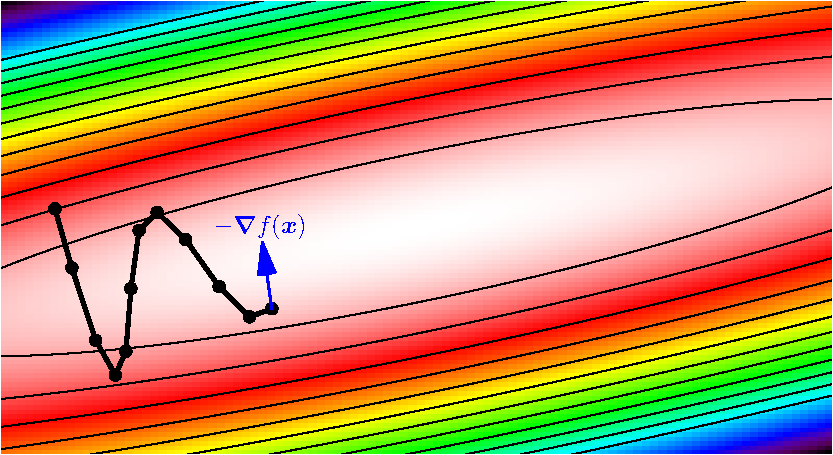
\includegraphics[width=0.9\linewidth]{momentumDynamics-23}
\end{center}
\keywords{SGD, momentum, step size, RMSProp, Adam, learning-rate schedules}
%%%%%%%%%%%%%%%%%%%%%%% Next Slide %%%%%%%%%%%%%%%%%%%%%%%
\renewcommand{\Outline}{%
\begin{slide}
\section[1]{Outline}

\begin{minipage}{12cm}\raggedright
  \begin{enumerate}\squeeze
    \outlineitem{SGD}{sgd}
    \outlineitem{Momentum}{momentum}
    \outlineitem{Loss Landscapes}{landscapes}
  \end{enumerate}
\end{minipage}\hfill
\begin{minipage}{10cm}
  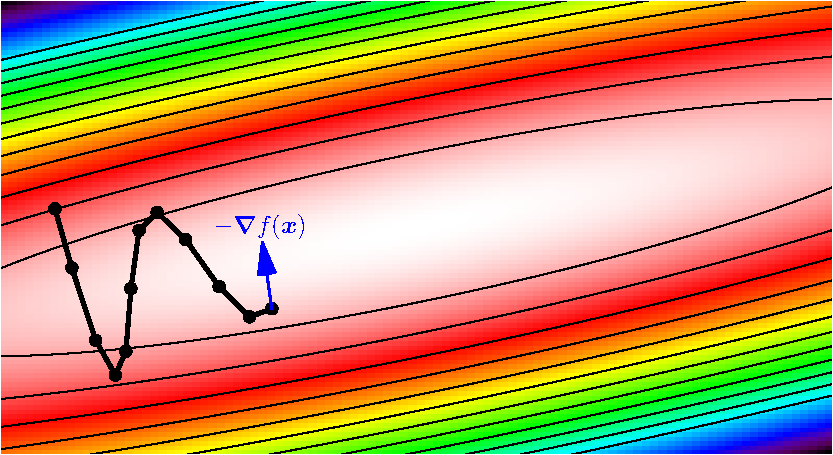
\includegraphics[width=10cm]{momentumDynamics-23}
\end{minipage}
\end{slide}
\addtocounter{outlineitem}{1}
}

\setcounter{outlineitem}{1}

%%%%%%%%%%%%%%%%%%%%%%% Next Slide %%%%%%%%%%%%%%%%%%%%%%%
\Outline % Motivation
\toptarget{firstoutline}
%%%%%%%%%%%%%%%%%%%%%%% Next Slide %%%%%%%%%%%%%%%%%%%%%%%

\begin{slide}
\section{The Next Step}

\begin{PauseHighLight}
  \begin{itemize}
  \item In most machine learning problems we design a network and a
    loss function\pause
  \item The rest requires simple optimisation\pause
  \item Although Newton and Quasi-Newton methods ensure rapid
    convergence for many tasks this apparent advantage is illusory\pause
  \item Since the rise of deep learning, gradient descent and its
    variants have become dominant\pause    
  \end{itemize}
\end{PauseHighLight}

\end{slide}

%%%%%%%%%%%%%%%%%%%%%%% Next Slide %%%%%%%%%%%%%%%%%%%%%%%

\begin{slide}
\section{Mini-Batch Learning}

\begin{PauseHighLight}
  \begin{itemize}
  \item Rather than computing the gradient of the loss function, e.g.
    \begin{align*}
      \grad L_{\mathcal{D}}(\bm{w}) = \frac{1}{|\mathcal{D}|}\grad \sum_{(\bm{x},y)\in\mathcal{D}}
      L\!\left( \strut f(\bm{x}|\bm{w}), y \right)\pause
    \end{align*}
  \item We often compute an approximation
    \begin{align*}
      \grad L_{\mathcal{B}}(\bm{w})
      = \frac{1}{|\mathcal{B}|}\grad \sum_{(\bm{x},y)\in\mathcal{B}}
      L\!\left( \strut f(\bm{x}|\bm{w}), y \right)
    \end{align*}
  \item where $\mathcal{B}\subset\mathcal{D}$ is a randomly sampled
    subset of the training set\pause
  \item Usually $|\mathcal{B}| \ll |\mathcal{D}|$\pause
  \end{itemize}
\end{PauseHighLight}

\end{slide}

%%%%%%%%%%%%%%%%%%%%%%% Next Slide %%%%%%%%%%%%%%%%%%%%%%%

\begin{slide}
  \section{Stochastic Gradient Descent}

\begin{PauseHighLight}
  \begin{itemize}
  \item Stochastic gradient descent (SGD) follows the gradient of
    mini-batches\pause
  \item Computationally this is efficient because it is much quicker to
    compute $\grad L_{\mathcal{B}}(\bm{w})$ than $\grad
    L_{\mathcal{D}}(\bm{w})$\pause
  \item The batch gradients add noise (are stochastic) as we are only
    sampling the dataset\pause
  \item This noise might help escape local-minima\pause{} (but I'm not sure
    there is compelling evidence for this)\pauseb
  \item Taking many smaller steps of approximate gradients reduces the
    likelihood of divergence\pause
  \end{itemize}
\end{PauseHighLight}


\end{slide}

%%%%%%%%%%%%%%%%%%%%%%% Next Slide %%%%%%%%%%%%%%%%%%%%%%%

\begin{slide}
  \section{Automatic Differentiation}

\begin{PauseHighLight}
  \begin{itemize}
  \item For gradient descent we need to compute the gradient\pause
  \item For most of my life this was just a pain\pause
  \item You guys have it easy, modern deep learning frameworks do this
    for you automatically\pause
  \item This is a \textit{game changer}!\pause{}  We are no longer afraid of
    large models\pause
  \item We can differentiate through algorithms allowing us to
    train incredibly sophisticated networks\pause
  \end{itemize}
\end{PauseHighLight}


\end{slide}

%%%%%%%%%%%%%%%%%%%%%%% Next Slide %%%%%%%%%%%%%%%%%%%%%%%

\begin{slide}
\section{Convergence}

\begin{PauseHighLight}
  \begin{itemize}
  \item Asymptotic convergence of gradient descent (and SGD) is slower
    than quasi-Newton methods\pause
  \item But there are three reasons why we don't really care\pause
    \begin{itemize}
    \item For complex models we spend a lot of time before we are
      close to a quadratic minimum where asymptotic convergence kicks in\pause
    \item These days we often use ReLUs (rectified linear units) which are not differentiable at 0.  The convergence we discussed depends on a
      Taylor expansion that assumes a smooth (twice differentiable) loss\pause
    \item We want to minimise the generalisation error, but are only
      minimising a poor surrogate, namely the training error\pause
    \end{itemize}
        
  \end{itemize}
\end{PauseHighLight}

\end{slide}



%%%%%%%%%%%%%%%%%%%%%%% Next Slide %%%%%%%%%%%%%%%%%%%%%%%
\Outline %  Momentum
%%%%%%%%%%%%%%%%%%%%%%% Next Slide %%%%%%%%%%%%%%%%%%%%%%%

\begin{slide}
\section[-2]{Recap: One Step Size, Many Curvatures}
\begin{rightImage}{eigspec}
\begin{PauseHighLight}
  \begin{itemize}
  \item The Hessian has a spectrum of eigenvalues: some directions are
    steep, others nearly flat\pause
  \item One step size $r$ must satisfy $r<2/\lambda_{\max}$, or we
    diverge (and quickly get NaN errors)\pause
  \item The flat directions then shrink by only about $1-1/\kappa$ per
    step\pause
  \item This seems hopelessly slow\pauseb, yet plain SGD (nearly always
    with momentum) is widely used in deep learning\pauseb
  \end{itemize}
\end{PauseHighLight}
\end{rightImage}
\end{slide}

%%%%%%%%%%%%%%%%%%%%%%% Next Slide %%%%%%%%%%%%%%%%%%%%%%%

\begin{slide}
  \section{Momentum}

  \begin{PauseHighLight}
    \begin{itemize}
    \item In high dimensions we zig-zag:
      \begin{itemize}
      \item stepping consistently in directions with low curvature
      \item jumping backwards and forwards past the minimum in
        directions with high curvature\pause
      \end{itemize}
    \item By introducing ``momentum'' we can increase our steps in
      low curvature directions and decrease them in high curvature directions
      \begin{align*}
        \bm{v}(t+1) &= \gamma \, \bm{v}(t) -  r\, \grad f(\bm{x}(t))\\
        \bm{x}(t+1) &= \bm{x}(t) + \bm{v}(t+1)\pause
      \end{align*}
      $0<\gamma<1$ sets how much velocity is kept ($1-\gamma$ acts as friction)\pauseb 
    \end{itemize}
  \end{PauseHighLight}


\end{slide}


%%%%%%%%%%%%%%%%%%%%%%% Next Slide %%%%%%%%%%%%%%%%%%%%%%%

\begin{slide}
\section{Gradient Descent with Momentum}

\pauselevel{=1:}
\pb\pause\pauselevel{=1}
\begin{center}
  \multipdf[width=\linewidth]{momentumDynamics}\pause
\end{center}
\end{slide}

%%%%%%%%%%%%%%%%%%%%%%% Next Slide %%%%%%%%%%%%%%%%%%%%%%%

\begin{slide}
\section[-2]{Nesterov Momentum}

\begin{PauseHighLight}\squeeze
  \begin{itemize}
  \item Nesterov's variant takes the gradient where momentum is about to
    carry us
    \begin{align*}
      \bm{v}(t+1) &= \gamma\,\bm{v}(t) - r\,\grad f\bigl(\bm{x}(t)+\gamma\,\bm{v}(t)\bigr)\\
      \bm{x}(t+1) &= \bm{x}(t) + \bm{v}(t+1)\pause
    \end{align*}
  \item With well-tuned momentum the number of steps needed scales as
    $\sqrt{\kappa}$ rather than $\kappa$\pause
  \item The convergence is still \emph{linear}: momentum fixes the
    condition number, not the order of convergence\pause
  \item On convex problems Nesterov reaches error $O(1/t^2)$ rather
    than $O(1/t)$, the best any gradient method can do (much more in
    COMP6260, Optimisation for Machine Learning)\pause
  \end{itemize}
\end{PauseHighLight}
\end{slide}

%%%%%%%%%%%%%%%%%%%%%%% Next Slide %%%%%%%%%%%%%%%%%%%%%%%

\begin{slide}
  \section{Adaptive Methods}

  \begin{PauseHighLight}
    \begin{itemize}
    \item A major difficulty of high dimensional optimisation is the
      existence of different scales\pause
    \item That is, there are some directions where we have to move a
      lot (low curvature), while other directions we have to make small
      steps\pause
    \item In adaptive methods we use a dynamic algorithm to rescale
      the step size of each parameter (weight)\pause
    \item We can think of this as a ``regularisation'' that makes our
      basins of attraction more spherical\pause
    \end{itemize}
  \end{PauseHighLight}

\end{slide}

%%%%%%%%%%%%%%%%%%%%%%% Next Slide %%%%%%%%%%%%%%%%%%%%%%%

\begin{slide}
\section[-2]{Rescaling Co-ordinates}

\pb\pauselevel{=1: 4}\pause\pauselevel{=1}
\begin{center}
  \multipdf[width=0.6\linewidth]{rescaleWeights}\pause
\end{center}
\end{slide}

%%%%%%%%%%%%%%%%%%%%%%% Next Slide %%%%%%%%%%%%%%%%%%%%%%%

\begin{slide}
\section[-2]{RMSProp}

\begin{PauseHighLight}
  \begin{itemize}\squeeze
  \item Rescale each coordinate by the typical size of its gradient\pause
  \item Keep a running average of the squared gradients
    \begin{align*}
      S_i(t+1) = (1-\gamma)\, S_i(t) + \gamma \left(
      \pd{L_{\mathcal{B}}(\bm{w}(t))}{w_i(t)} \right)^2\pause
    \end{align*}
  \item and divide the step by its square root
    \begin{align*}
      w_i(t+1) = w_i(t) - \frac{r}{\sqrt{S_i(t+1)}+\epsilon}\,
      \pd{L_{\mathcal{B}}(\bm{w}(t))}{w_i(t)}\pause
    \end{align*}
  \item Steep directions take small steps and flat ones large steps:
    each weight moves about $r$ per step, whatever the scale of the loss\pause
  \end{itemize}
\end{PauseHighLight}
\end{slide}

%%%%%%%%%%%%%%%%%%%%%%% Next Slide %%%%%%%%%%%%%%%%%%%%%%%

\begin{slide}
\section[-2]{Adding in Momentum}

\begin{PauseHighLight}
  \begin{itemize}
  \item RMSProp has no momentum (one argument is that rescaling has
    already ``regularised the landscape'')\pause
  \item Nevertheless we can learn a momentum term
    {\small
    \begin{align*}
      M_i(t+1)
      &= (1-\beta)\,M_i(t) + \beta \,
        \pd{L_{\mathcal{B}}(\bm{w}(t))}{w_i(t)}
      \\
      S_i(t+1)
      &= (1-\gamma)\,S_i(t) + \gamma \,
        \left( \pd{L_{\mathcal{B}}(\bm{w}(t))}{w_i(t)} \right)^2\pause
    \end{align*}}
  \item Starting from $M_i(0)=S_i(0)=0$ biases these averages towards zero at first, which we correct
    \begin{align*}
      \hat{M}_i(t+1) &= \frac{M_i(t+1)}{1-(1-\beta)^{t+1}}
      &
        \hat{S}_i(t+1) &= \frac{S_i(t+1)}{1-(1-\gamma)^{t+1}}\pause
    \end{align*}
 \end{itemize}
\end{PauseHighLight}

\end{slide}

%%%%%%%%%%%%%%%%%%%%%%% Next Slide %%%%%%%%%%%%%%%%%%%%%%%

\begin{slide}
\section{ADAM}

\begin{PauseHighLight}
  \begin{itemize}\squeeze
  \item Adaptive Moment Estimation (Adam) adapts the scale of the
    parameters, but also uses momentum\pause
  \item Update weights
    \begin{align*}
      w_i(t+1) = w_i(t) - \frac{r}{\sqrt{\hat{S}_i(t+1)} + \epsilon}\,
      \hat{M}_i(t+1)\pause
    \end{align*}
  \item Adam and its variants are very successful in deep learning: a
    network often learns with Adam when it would not with SGD\pause
  \item \emph{AdamW} applies weight decay directly to the weights,
    $w_i \leftarrow w_i - r\,\eta\,w_i$, rather than through the loss,
    where Adam's rescaling would weaken it; the default for transformers\pause
  \end{itemize}
\end{PauseHighLight}

\end{slide}

%%%%%%%%%%%%%%%%%%%%%%% Next Slide %%%%%%%%%%%%%%%%%%%%%%%

\begin{slide}
\section[-2]{Covariant Equations}

\begin{PauseHighLight}
  \begin{minipage}{0.6\linewidth}
      \begin{itemize}
      \item Vector arithmetic, (matrix multiplication, addition,
        multiplying by a scale, computing gradients) has a covariant property that it is
        invariant to the coordinate system\pause
      \item That is we can translate and rotate our coordinates and get
        the same result\pause
      \item That is not true of element-wise multiplication of
        vectors\pause
      \item Many ML algorithms do this (including RMSProp and Adam), but
        they aren't invariant if we rotate our coordinates\pause
      \end{itemize}
    \end{minipage}\hfil
    \begin{minipage}{0.35\linewidth}
      \begin{center}
        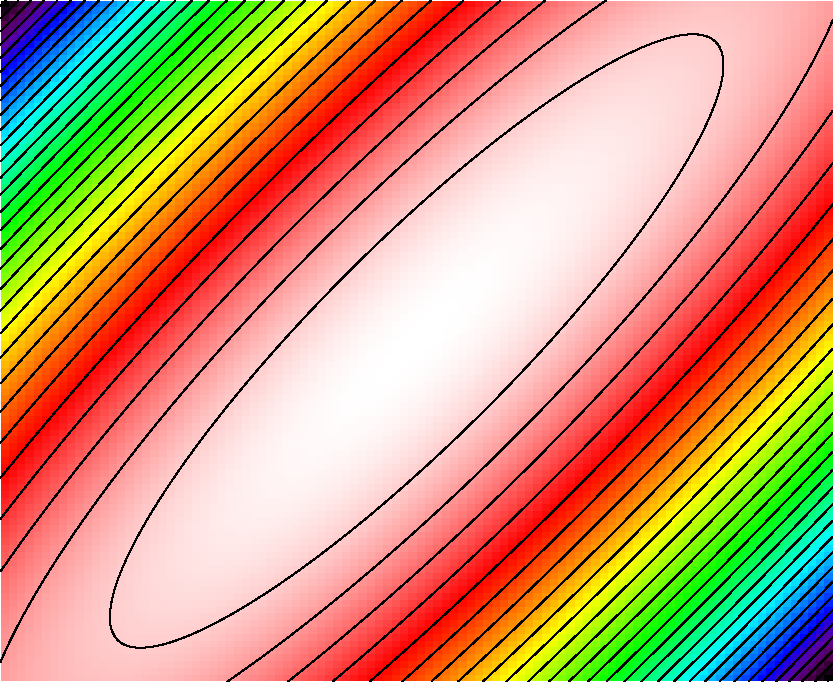
\includegraphics[width=\linewidth]{correlatedWeights}\pauseb\\
        Can't rescale coordinates\pauseb
      \end{center}
    \end{minipage}
\end{PauseHighLight}

\end{slide}


%%%%%%%%%%%%%%%%%%%%%%% Next Slide %%%%%%%%%%%%%%%%%%%%%%%

\begin{slide}
  \section{Correlated Weights}

  \begin{rightImage}{correlatedWeights}
    \begin{PauseHighLight}
      \begin{itemize}
      \item Correlated weights will lead to skewed valleys\pause
      \item Adaptive methods would be more efficient if they were
        rotationally invariant\pause
      \item However, this would slow down the algorithm\pause
      \item ADAM is a compromise between speed of implementation and
        effectiveness\pause
      \end{itemize}
    \end{PauseHighLight}

  \end{rightImage}

\end{slide}


%%%%%%%%%%%%%%%%%%%%%%% Next Slide %%%%%%%%%%%%%%%%%%%%%%%
\Outline %  Loss Landscape
%%%%%%%%%%%%%%%%%%%%%%% Next Slide %%%%%%%%%%%%%%%%%%%%%%%

\begin{slide}
\section[-2]{Loss Landscape}

\begin{PauseHighLight}
  \begin{itemize}\squeeze
  \item A useful concept for understanding optimisation is the loss
    landscape\pause
  \item For every value of the weights $\bm{w}$ there is some loss
    associated with it\pause
  \item Note that this landscape is very high dimensional, so our
    intuition can be a bit misleading\pause
  \item The landscape is also huge
  \end{itemize}
  \begin{center}
    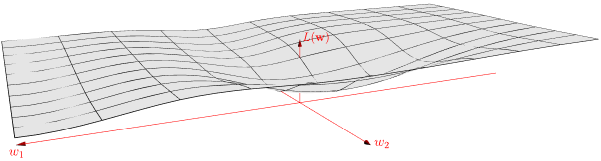
\includegraphics[width=0.9\linewidth]{lossLandscape.png}\pause
  \end{center}
\end{PauseHighLight}

\end{slide}

%%%%%%%%%%%%%%%%%%%%%%% Next Slide %%%%%%%%%%%%%%%%%%%%%%%

\begin{slide}
\section{Global and Local Minima}

\begin{PauseHighLight}
  \begin{itemize}
  \item Our objective is to minimise our loss\pause
  \item This would mean finding the global minimum\pause
  \item For non-convex losses no efficient algorithm is guaranteed to find
    the global minimum\pause
  \item The best we can hope is to find a local minimum by doing
    gradient descent\pause
  \item In practice, our landscapes are so large that we are probably
    unable to find even a local minimum\pause
  \end{itemize}
\end{PauseHighLight}

\end{slide}

%%%%%%%%%%%%%%%%%%%%%%% Next Slide %%%%%%%%%%%%%%%%%%%%%%%

\begin{slide}
\section{Noisy Optimisation}

\begin{PauseHighLight}
  \begin{itemize}
  \item Because we are using mini-batches we aren't actually following
    the correct gradients\pause
  \item If we reduce our step size then our average gradient is closer
    to the true gradient\pause
  \item Thus our optimisation is inherently noisy\pause
  \item At least for deep learning there is no evidence that the
    weights stop changing even after learning for a huge amount of time\pause
  \end{itemize}
\end{PauseHighLight}

\end{slide}


%%%%%%%%%%%%%%%%%%%%%%% Next Slide %%%%%%%%%%%%%%%%%%%%%%%

\begin{slide}
\section{Valleys in Valleys in Valleys}

\begin{PauseHighLight}
  \begin{itemize}
  \item My view of the loss landscape is that we have valleys inside
    bigger valleys inside bigger valleys, and so on\pause
  \item If our noise is high (we use large step size), we can navigate
    away from local valleys and move towards the big valley\pause
  \item But, we can't explore the small valleys\pause
  \item Often when the rate of improvement slows down, practitioners
    will reduce their learning rate by a factor of 10 and the rate of
    improvement jumps up\pause
  \item Some practitioners cycle through raising and lowering their
    learning rates which may speed up convergence\pause
  \end{itemize}
\end{PauseHighLight}

\end{slide}

%%%%%%%%%%%%%%%%%%%%%%% Next Slide %%%%%%%%%%%%%%%%%%%%%%%

\begin{slide}
\section[-2]{Reducing the Step Size}
\pb
\pause
\pauselevel{=1}
\begin{center}
  \multipdf[width=0.7\linewidth]{valleyInValley}\pause
\end{center}
\begin{center}
  \multipdf[width=0.7\linewidth]{OUprocess}\pause
\end{center}

\end{slide}

%%%%%%%%%%%%%%%%%%%%%%% Next Slide %%%%%%%%%%%%%%%%%%%%%%%

\begin{slide}
\section[-2]{Learning-Rate Schedules}

\begin{PauseHighLight}
  \begin{itemize}\squeeze
  \item Large $r$ early: noisy steps cross the small valleys and find the
    big ones\pause
  \item Small $r$ late: settle into a valley\pause
  \end{itemize}
  \begin{center}
    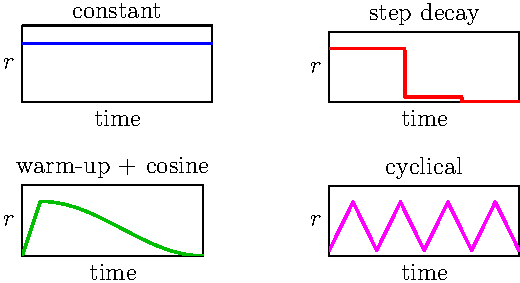
\includegraphics[width=0.7\linewidth]{lrSchedules}\pause
  \end{center}
  \begin{itemize}\squeeze
  \item A short warm-up stops the first steps diverging before Adam's
    running averages have settled; common for transformers\pause
  \end{itemize}
\end{PauseHighLight}
\end{slide}


%%%%%%%%%%%%%%%%%%%%%%% Next Slide %%%%%%%%%%%%%%%%%%%%%%%

\begin{slide}
\section[-2]{Symmetries}

\pb
\begin{itemize}
\item When training neural networks (deep or shallow) there are
  typically many symmetries\pauseh
\item Examples come from permuting the neurons (or filters in CNNs)
  within a layer, together with their weights\pauseh
  \begin{center}
    \multipdf[width=0.6\linewidth]{permutationSymmetry}\pause
  \end{center}
\end{itemize}

\end{slide}

%%%%%%%%%%%%%%%%%%%%%%% Next Slide %%%%%%%%%%%%%%%%%%%%%%%

\begin{slide}
\section[-2]{More Symmetries}

\begin{PauseHighLight}
  \begin{itemize}
  \item With $n$ hidden nodes there are $n!$ symmetries\pause
  \item For odd activation functions such as $\tanh$, multiplying all the
    input and output weights of a node by $-1$ gives the same network\pause
  \item There are also continuous symmetries.  For linear networks
    with two layers performing a mapping $\mat{W}_2 \mat{W}_1$ then
    for any invertible matrix $\mat{U}$ (where
    $\mat{U}\mat{U}^{-1}=\mat{I}$)
    \begin{align*}
      \mat{W}_2 \mat{W}_1 = \mat{W}_2  \,\mat{I} \, \mat{W}_1\pause
      = \mat{W}_2 \,(\mat{U}\,\mat{U}^{-1}) \mat{W}_1\pauseb
     = (\mat{W}_2 \,\mat{U})\,(\mat{U}^{-1} \mat{W}_1)\pauseb
    \end{align*}
    so a network with weights $\mat{W}_2'=\mat{W}_2 \,\mat{U}$ and
    $\mat{W}_1'=\mat{U}^{-1}\mat{W}_1$ will perform the same mapping\pause
  \item There will be a huge space of equivalent networks\pause
  \end{itemize}
\end{PauseHighLight}

\end{slide}

%%%%%%%%%%%%%%%%%%%%%%% Next Slide %%%%%%%%%%%%%%%%%%%%%%%

\begin{slide}
  \section[-2]{Skip Connections}

  \pb\pauselevel{=1 :30}\pause\pauselevel{=1}
  \begin{center}
    \multipdf[width=0.8\linewidth]{skipConnections}\pause
  \end{center}
  \begin{itemize}
  \item Breaks permutation symmetry\pause. Used in Resnets,
    transformer, etc.\pause
  \end{itemize}
\end{slide}



%%%%%%%%%%%%%%%%%%%%%%% Next Slide %%%%%%%%%%%%%%%%%%%%%%%

\begin{slide}
\section[-2]{Symmetries}

\pb\pause
\begin{minipage}{0.6\linewidth}
  \begin{itemize}
\item The landscape potentially has a huge manifold with the same
  losses (neutral network)\pauseh
\item Find solution close to start\pauseh \pauselevel{=30}
\item We should think of optimisation more as a process of
  travelling than a process of arriving\pauseh
\item Of course even if we do minimise our loss we are not
  guaranteed to minimise our generalisation performance\pauseh
\end{itemize}\hfill
\end{minipage}
\begin{minipage}{0.35\linewidth}\pauselevel{=3}
  \begin{flushright}
    \multipdf[width=0.85\linewidth]{symmetryLoss}\pause
  \end{flushright}
\end{minipage}

\end{slide}

%%%%%%%%%%%%%%%%%%%%%%% Next Slide %%%%%%%%%%%%%%%%%%%%%%%

\begin{slide}
\section{Lessons}

\begin{PauseHighLight}
  \begin{itemize}
  \item SGD together with automatic differentiation has revolutionised
    machine learning\pause
  \item There are a number of techniques to get the step size
    right\pause: momentum (and Nesterov)\pauseb, adaptive step sizes
    (RMSProp)\pauseb, Adam and AdamW\pauseb, learning-rate schedules\pauseb
  \item Still need to understand that we are exploring a huge and
    complex loss landscape\pause
  \item What works is problem specific\pause{} (as always)\pauseb
  \end{itemize}
\end{PauseHighLight}

\end{slide}

%%% Local Variables:
%%% TeX-master: "lectures"
%%% End:

\end{document}
